\section{Result and analysis}
Here we apply our algorithm to a variety of images, ranging from purely synthetic images to full-color photographs that include complex textures. According tor test result, our algorithm can handle different size of mask and different kinds of texture.

We test our algorithm in three scenarios, which includes image text removal, image object removal and image detail restoration. The following part will use some case to illustrate and analysis the result.

\subsection*{Image text removal}
In our daily life, we may often meet with image covered by text such as brand and advertisement. Given the mask which cover the whole text on the image, our algorithm can remove the text.

The example is shown in $Figure.3$, with the mask which cover the whole red text on the image, this algorithm will remove the whole red text. 
\begin{figure}
	\centering
	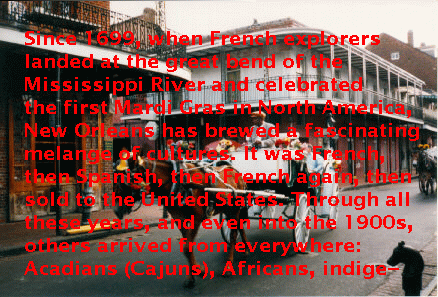
\includegraphics[width=0.9\linewidth]{horse_car.png}\\\ \\
	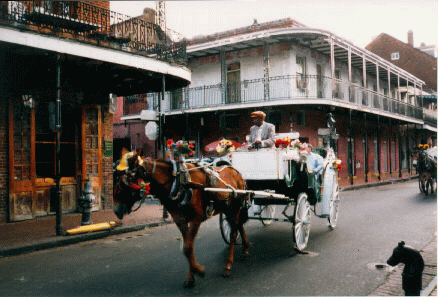
\includegraphics[width=0.9\linewidth]{horse_car_result.png}
	\caption{\textbf{Image text removal}. The original image and inpainted image}
\end{figure}

\subsection*{Image object removal}
Compared with previous field model \etal\cite{cvpr10mrf, ijcv09}, which can not handle large mask well, our algorithm can successfully inpainting large mask. The result is shown in the $Figure.4$. 
\begin{figure}
	\centering
	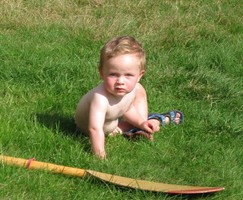
\includegraphics[width=0.9\linewidth]{kid.jpg}\\\ \\
	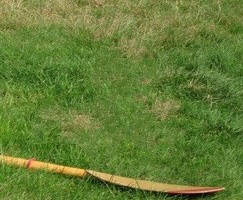
\includegraphics[width=0.9\linewidth]{kid_result.jpg}
	\caption{\textbf{Image object removal}. The original image and inpainted image}
\end{figure}

\subsection*{Image detail restoration}
We may get some disrupted images such as old photos. The result of the image detail restoration is shown in $Figure.5$. If observed inpainted image carefully, you may find some inpainting trace on it, but it dose not matter for the final result. As the result shows, it works well.
\begin{figure}
	\centering
	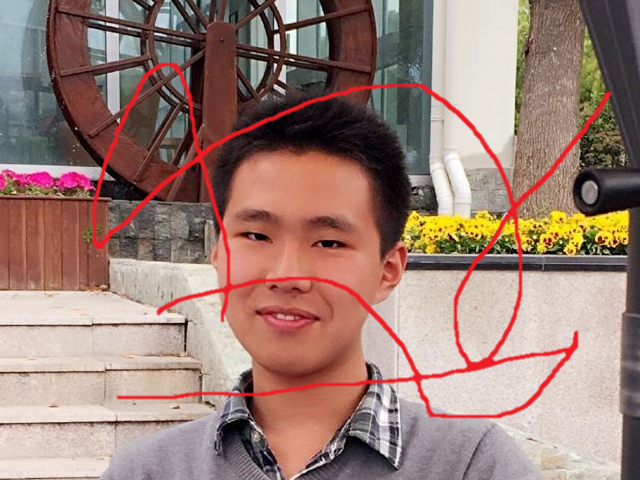
\includegraphics[width=0.9\linewidth]{zouyikai.png}\\\ \\
	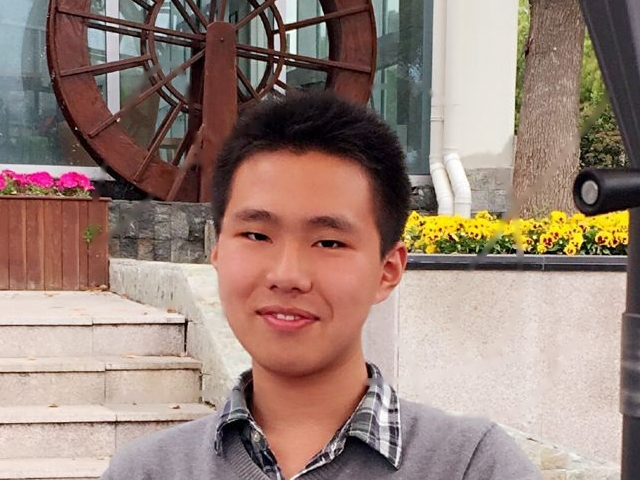
\includegraphics[width=0.9\linewidth]{zouyikai_result.png}
	\caption{\textbf{Image detail restoration}. The original image and inpainted image}
\end{figure}